\section{Laboratory work implementation}

\subsection{Tasks and Points}

Basic Level (grade 5 || 6):

-    Draw 5 lines of different colors and weights

-    Draw 2 Bezier curves

-    Draw 4 plane objects (ex. circle, square, pie, polygon...) of different colors, weights, filled and not

-    Draw 2 different objects using mouse

Normal Level (grade 7 || 8):

-    Realize the tasks from Basic Level.

-    Hook keyboard input. Add 2 different keyboard combinations that will change mouse ability to draw objects (ex. on Ctrl+C will draw circles, on Alt+R will continue to draw circles but of read color)
    Draw a Bezier curve using mouse

Advanced Level (grade 9 || 10):

-    Realize the tasks from Normal Level.

-    Use mouse as an eraser (chosen option): eraser with adjustable width





\subsection{Laboratory work analysis}
Repository:

https://github.com/StasBizdiga/WP

\subsection{Proving my work}

Basic level:


\includegraphics[scale=0.55]{pic_1} \\

- All the required things are drawn.

------------------------------------ \\

Normal level: \\

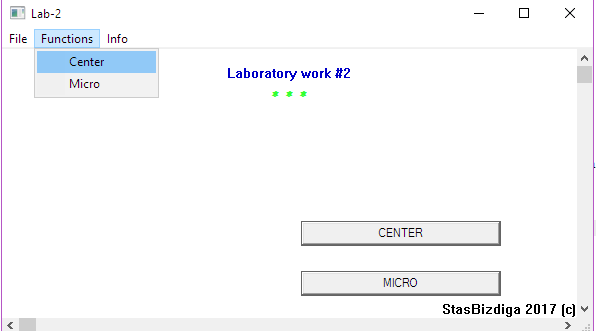
\includegraphics{pic_2} \\

Bezier curves are being modified by:

Top Curve: Shift+RClick / Shift+LClick

Bottom Curve: Ctrl+RClick / Ctrl+LClick 


------------------------------------------ \\


Advanced level / Other features:

- Weight is adjustable by numpad " + " and " - " 

(Thus by selecting the white color and using this feature we obtain the dynamically adjustable eraser required in Advanced level)

- Pen/Border/Fill Color is chosen from menu (see more below in the menus description)


-------------------------------------------------- \\

Hotkeys cheat-sheet:

- Pressing Del clears the screen.

- Pressing Esc deselects any tool currently enabled.

- Pressing Space sets Fill on/off.

- Pressing +/- adjusts weight. 

-------------------------------------------------- \\

Menus notes:

- Fill option may be on/off by either clicking it in menu or pressing Space.

- Colors and painting tools are selection based - choosing an option enables it and disables the conflicting ones. \\


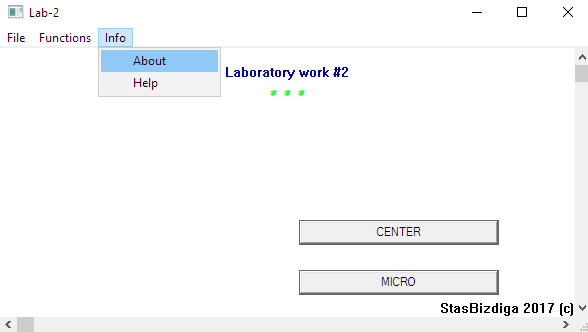
\includegraphics{pic_3} \\

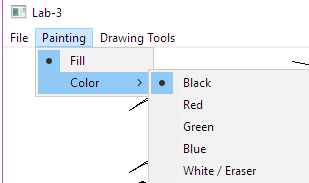
\includegraphics{pic_4} \\

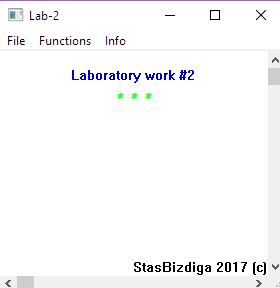
\includegraphics{pic_5} 



\clearpage